% Definição do tamanho da letra, folha e estilo.
\documentclass[12pt, a4paper]{article}

% Definição de pacotes.
%% Padrão UTF-8.
%% Texto brasileiro.
%% Identação dos parágrafos.
%% Adição de imagens.
%% Geometria da página de acordo com a ABNT.
\usepackage[utf8]{inputenc}
\usepackage[brazil]{babel}
\usepackage{indentfirst}
\usepackage{graphicx}
\usepackage{float}
\usepackage{geometry}
\geometry{a4paper, left = 3cm, right = 3cm, top = 3cm, bottom = 3cm}

% Numeração da página.
\pagenumbering{arabic}

% Path das imagens.
\graphicspath{{./img/}}

\title{\textbf{Cache 2-vias}}
\author{
	Guimarães, João Guilherme M.\\
	\texttt{joaog95@live.com}
}
\date{\today}

\begin{document}
	% Escrever o título, autor e data.
	\maketitle
	
	% Espaçamento vertical
	\vspace{1cm}
	
	\section{Introdução}
	
	\par A cache associativa de 2-vias é um \textit{trade-off} entre a cache diretamente mapeada e a totalmente associativa. Seu funcionamento consiste em dividir a cache em \textit{sets} de dimensão 2, o que possibilita uma maior taxa de acerto quando comparada a diretamente mapeada e uma redução do custo energético em relação a totalmente associativa.

	\vspace{\baselineskip}
	
	\begin{figure}[H]
		\centering
		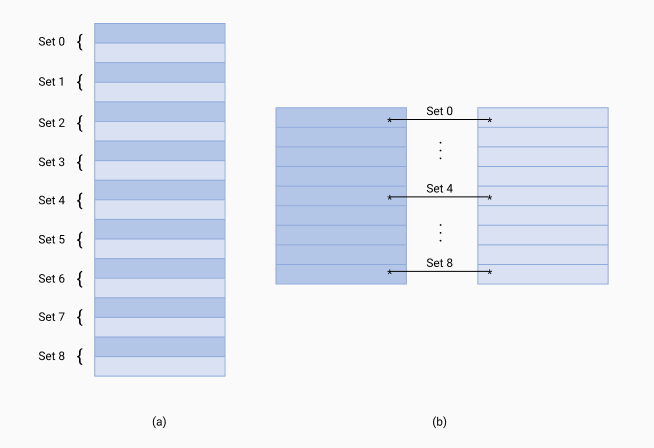
\includegraphics[width=15.3cm]{./cache}
		\caption{Cache 2-vias}
		\label{fig: cache 2-vias}
	\end{figure}

	\par Na figura \ref{fig: cache 2-vias}, é representado as possíveis abstrações de uma cache de 2-vias, sendo que em \textit{a} é utilizado um único módulo de memória, enquanto em \textit{b}, são utilizados dois módulos. Neste projeto foi utilizado a abstração \textit{a}.

	\section{Objetivos}
	
	\par Implementação de uma cache associativa de 2-vias, com utilização do arquivo MIF e realizar a leitura e escrita utilizando o display de 7-segmentos.
	
	\section{Material}
	
	\par Para realização desta prática, foi utilizado os seguintes equipamentos e softwares:
	
	\begin{itemize}
		\item ModelSim 10.1d;
		\item Quartus 13.0sp1;
		\item FPGA EP2C35F672C6 e
		\item Kernel Linux / SO Deepin 15.11.
	\end{itemize}
	
    \section{Desenvolvimento}
    
	\par O primeiro passo para o desenvolvimento do projeto, foi a detalhação das especificações da cache, que são:

	\vspace{\baselineskip}

	\begin{itemize}
		\item Associatividade: 2-vias;
		\item Tamanho da palavra: 16 bits;
		\item Tamanho do bloco: 2 palavras e
		\item Tamanho da memória: 16 palavras.
	\end{itemize}

	\vspace{\baselineskip}

	\par A partir do detalhamento acima, foi proposto a abstração \textit{a} da figura \ref{fig: cache 2-vias}, pois o desenvolvimento do código seria facilitado, devido a necessidade da comunicação entre as caches. O próximo passo, foi a divisão dos campos do endereçamento, dado por:
	
	\vspace{\baselineskip}
	
	\begin{itemize}
		\item TAG: 8 - Index - Block Offset = 5
		\item Index: $ln(8/2) = ln(2^{2}) = 2$ bits
		\item Block Offset: $ln($Palavras por bloco$) = 1$ bit
	\end{itemize}

	\vspace{\baselineskip}

	\par Com a obtenção do tamanho da TAG, foi definido as seguintes divisões para a cache:
	
	\vspace{\baselineskip}
	
	\begin{itemize}
		\item Valid: 1 bit;
		\item Dirty: 1 bit;
		\item Tag: 5 bits;
		\item Bloco: 16 bits e
		\item LRU: 1 bit
	\end{itemize}
    
    \vspace{\baselineskip}
    
    \par Para facilitar o entendimento da estrutura acima, foi criado o arquivo MIF.xlsx que é exibido na figura a seguir.
    
    \vspace{\baselineskip}
    
    \begin{figure}[H]
    	\centering
    	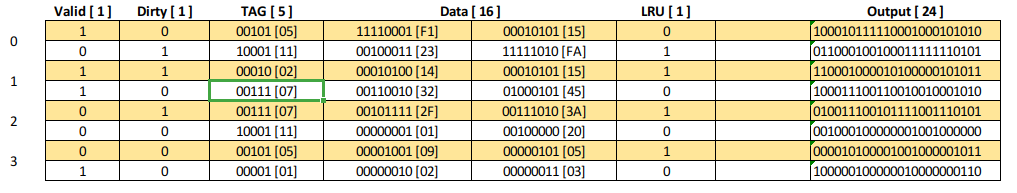
\includegraphics[width=15.3cm]{./cache_definitions}
    	\caption{Estrutura da Cache}
    	\label{fig: cache definitios}
    \end{figure}
    
	\section{Simulação}
	
	\par Como discutido em sala, a simulação poderia ser simplificada devido a correta execução do código na placa da Altera, sendo assim, foi simulado a leitura com sucesso do endereço $13_{16}$ (Set 1, Bloco 0), a escrita no mesmo endereço utilizando o dado $51_{16}$ e posteriormente a leitura do endereço $3A_{16}$ (Set 1, Bloco 1).
	
	\begin{figure}[H]
		\centering
		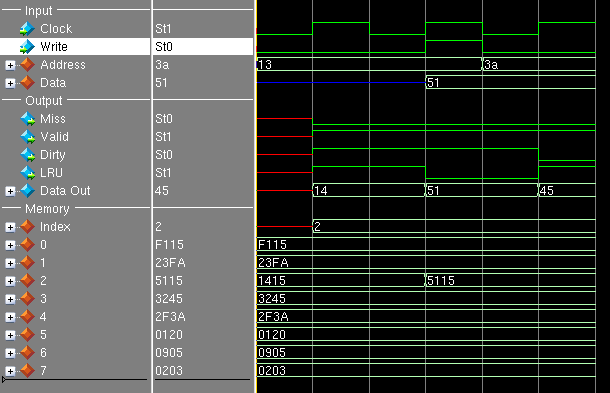
\includegraphics[width=15.3cm]{./Read_and_Write}
		\caption{Leitura e Escrita na Cache}
		\label{fig: Read and Write}
	\end{figure}
    
	\vspace{\baselineskip}
	
	\par \textit{Obs.: como o módulo para a exibição no display de 7-segmentos foi reaproveitado da prática anterior, sua simulação não foi refeita.}

	\section{Conclusão}
	
	\par Com a execução desta prática, foi possível entender melhor o funcionamento das políticas de pesquisa e inserção em uma cache de 2-vias e um entendimento dos problemas de assincronicidade do Clock em Verilog.

\end{document}
	